%%%
% Original author:
% Sean Bone
% http:// weblog.zumguy.com
%%%


% Use extarticle for the smaller font size:
% https://tex.stackexchange.com/questions/5339/how-to-specify-font-size-less-than-10pt-or-more-than-12pt
\documentclass[a4paper, 8pt]{extarticle}

% Multi-column layout
\usepackage{multicol}
% Manually set page margins
\usepackage[margin=0.5cm]{geometry}

% Manually set margins on lists
\usepackage{enumitem}
% Change list margins - https://tex.stackexchange.com/questions/10684/vertical-space-in-lists
\setlist{leftmargin=3mm, noitemsep}
% or \setlist{noitemsep} to leave space around whole list

\usepackage{amsmath}
\usepackage{siunitx}
\usepackage{mathtools}
\usepackage{amssymb}
\usepackage{graphicx}
\usepackage{bm}
%\usepackage[shortlabels]{enumitem}

% Additional Packages
\usepackage{comment}
\usepackage{graphicx}
\usepackage[export]{adjustbox}

%%%% Useful
% Negative margins on equations: \mkern-36mu
% Negative vertical spacing: \vspace{-0em}
% Split equations: \begin{multline} ... \\ ... \end{multline}


%%%% Change list margins
% https://tex.stackexchange.com/questions/97305/how-to-change-the-indentation-of-all-enumerates
%\setlist[enumerate,1]{leftmargin=0.5cm}
%\setlist[enumerate,2]{leftmargin=0.5cm}
%\setlist[itemize,1]{leftmargin=0.2cm}
%\setlist[itemize,2]{leftmargin=0.5cm}
%\setlist{nosep} % https://tex.stackexchange.com/questions/10684/vertical-space-in-lists


%%%% Title & author
\title{Robot Dynamics HS19}
\author{Thomas Bucher \\ \ \\ Based on Summary of Sean Bone \\ http://weblog.zumguy.com/ }
\date{ \today }

%%%% Custom commands
\newcommand{\mvec}[3]{  \prescript{}{\mathcal{#1}}{\bm{#2}}  _{#3} }
\newcommand{\mdvec}[3]{ \prescript{}{\mathcal{#1}}{\dot{\bm #2}} _{#3} }

\newcommand{\mrot}[2]{ \textbf{#1}_{ \mathcal{#2} } }
\newcommand{\mquat}[1]{ \bm{\xi}_{ \mathcal{#1} } }

\DeclareMathOperator{\atan2}{atan2}
\DeclareMathOperator{\taninv}{atan}
\DeclareMathOperator{\cosinv}{acos}
\DeclareMathOperator{\sgn}{sgn}


\begin{document}
\begin{multicols*}{3}

\maketitle


\section{Parametrizations}
\subsection{Position and velocity}
For every position parametrization, there is a linear mapping between linear velocities $\dot{\bm{r}}$ and derivatives of the representation $\dot{\bm{\chi}}$.\\
$\mdvec{}{r}{} = \bm{E}_P(\mvec{}{\chi}{P})\mdvec{}{\chi}{P},\; \mdvec{}{\chi}{P} = \bm{E}_P(\mvec{}{\chi}{P})^{-1}\mdvec{}{r}{}$\\

\noindent\textbf{Cartesian Coordinates:}\\
$\bm{E}_{P_c} = \mathbb{I}$\\
$\mvec{}{\chi}{P_c} = [x \quad y \quad z]^T,\; \mvec{A}{r}{} = [x \quad y \quad z]^T$\\

\noindent\textbf{Cylindrical coordinates:}\\
$\mvec{}{\chi}{P_z} = [\rho \quad \theta \quad z]^T,$\\
$\mvec{A}{r}{} = [\rho\cos\theta \quad \rho\sin\theta \quad z]^T$\\
$\bm E_{P_z} = 
\left[\begin{smallmatrix} 
\cos\theta  &  -\rho\sin\theta  &  0\\
\sin\theta  &  -\rho\cos\theta  &  0\\
0 & 0 & 1
\end{smallmatrix}\right]$\\
$\bm E_{P_z}^{-1} = 
\left[\begin{smallmatrix} 
\cos\theta  &  \sin\theta  &  0\\
-\sin\theta/\rho  &  \cos\theta/\rho  &  0\\
0 & 0 & 1
\end{smallmatrix}\right]$\\

\noindent\textbf{Spherical coordinates:}\\
$\mvec{}{\chi}{P_s} = [r \quad \theta \quad \phi]^T,$\\
$\mvec{A}{r}{} = [r\cos\theta\sin\phi \quad r\sin\theta\cos\phi \quad z]^T$\\
$\bm E_{P_s}=\left[\begin{smallmatrix} 
\cos\theta\sin\phi  &  -r\sin\phi\sin\theta  &  r\cos\phi\cos\theta \\
\sin\phi\sin\theta  &  r\cos\theta\sin\phi   &  r\cos\phi\sin\theta\\
\cos\phi  &  0  &  -r\sin\phi
\end{smallmatrix}\right]$\\
$\bm E_{P_s}^{-1}=\left[ \begin{smallmatrix} 
\cos\theta\sin\phi  &  \sin\phi\sin\theta  &  \cos\phi\\
-\sin\theta/(r\sin\phi)  &  \cos\theta/(r\sin\phi)  &  0\\
(\cos\phi\cos\theta)/r  &  (\cos\phi\sin\theta)/r  & -\sin\phi/r
\end{smallmatrix} \right]$

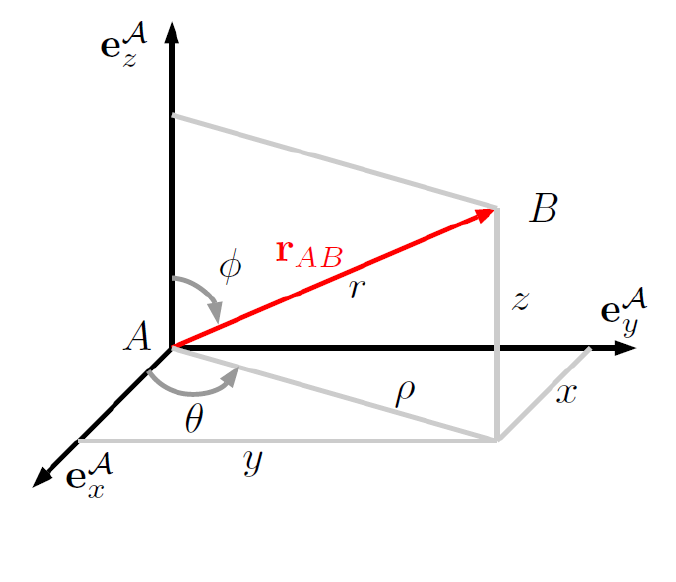
\includegraphics[width=0.85\linewidth]{images/Overview_Coordinates.PNG}

\subsection{Rotation}
%$\atan2(y,x) \coloneqq \taninv(\frac{y}{x})$, checking for correct quadrant.\\
$\mvec{A}{u}{} = \mrot{C}{AC} \cdot \mvec{C}{u}{} = \mrot{C}{AB}\mrot{C}{BC} \cdot \mvec{C}{u}{}$\\
$\mrot{C}{BA} = \mrot{C}{AB}^{-1} = \mrot{C}{AB}^T$\\
$\mrot{C}{AB}\mrot{C}{AB}^T=I_{n}$ (Orthogonality)

\noindent\textbf{Elementary rotations:}

$\textbf{C}_x = \left[\begin{smallmatrix}
1  &  0  &  0\\
0  & \cos\varphi  &  -\sin\varphi\\
0  & \sin\varphi  &  \cos\varphi
\end{smallmatrix}\right]$

$\textbf{C}_y = \left[\begin{smallmatrix}
\cos\varphi  &  0  &  \sin\varphi\\
0  &  1  &  0\\
-\sin\varphi  &  0  &  \cos\varphi
\end{smallmatrix}\right]$

$\textbf{C}_z = \left[\begin{smallmatrix}
\cos\varphi  &  -\sin\varphi &  0\\
\sin\varphi  &  \cos\varphi  &  0\\
0  &  0  &  1\\
\end{smallmatrix}\right]$

\noindent\textbf{Euler ZYZ} (proper) angles:\\
$\mvec{}{\chi}{R,ZYZ} = \left(\begin{smallmatrix}
\atan2(c_{23},c_{13})\\
\atan2(\sqrt{c_{13}^2 + c_{23}^2}, c_{33})\\
\atan2(c_{32}, -c_{31})
\end{smallmatrix}\right)$

\noindent\textbf{Euler ZXZ} (proper) angles:\\
$\mvec{}{\chi}{R,ZXZ} = \left(\begin{smallmatrix}
\atan2(c_{13},-c_{23})\\
\atan2(\sqrt{c_{13}^2 + c_{23}^2}, c_{33})\\
\atan2(c_{31}, c_{32})
\end{smallmatrix}\right)$

\noindent\textbf{Euler ZYX} (Tait-Bryan) angles:\\
$\mvec{}{\chi}{R,ZYX} = \left(\begin{smallmatrix}
\atan2(c_{21},c_{11})\\
\atan2(-c_{31}, \sqrt{c_{32}^2 + c_{33}^2})\\
\atan2(c_{32}, c_{33})
\end{smallmatrix}\right)$

\noindent\textbf{Euler XYZ} (Cardan) angles:\\
$\mvec{}{\chi}{R,XYZ} = \left(\begin{smallmatrix}
\atan2(-c_{23},c_{33})\\
\atan2(c_{13}, \sqrt{c_{11}^2 + c_{12}^2})\\
\atan2(c_{12}, -c_{11})
\end{smallmatrix}\right)$

\noindent\textbf{Angle-axis/Rotation-vector (non-minimal)}:\\
\vspace{-2em}
\begin{multline*}
\mkern-36mu
\mvec{}{\chi}{R,AA} = \left(\begin{smallmatrix}
\theta\\
\mvec{}{n}{}
\end{smallmatrix}\right),\,
\mvec{}{n}{} = \frac{1}{2\sin(\theta)}\cdot
\left(\begin{smallmatrix}
c_{32} - c_{23}\\
c_{31} - c_{13}\\
c_{21} - c_{12}
\end{smallmatrix}\right),\, \\
\theta = \cosinv(\frac{c_{11} + c_{22} + c_{33} - 1}{2}),\, \bm \varphi = \theta\cdot\textbf n (n unit)
\end{multline*}

\noindent\textbf{Unit Quaternions (non-minimal)}:\\
$\mvec{}{\chi}{R,quat} = \mvec{}{\xi}{} = \left(\begin{smallmatrix}
\xi \\
 \check{\mvec{}{\xi}{}}
\end{smallmatrix}\right),\,
 \mvec{}{\xi}{}^{-1} = \left(\begin{smallmatrix}
\xi \\
-\check{\mvec{}{\xi}{}}
\end{smallmatrix}\right)$\\
$\xi_0 = \cos(\theta/2),\quad \check{\mvec{}{\xi}{}} = \mvec{}{n}{}\cdot\sin(\theta/2)$

$\mkern-36mu
\mvec{}{\chi}{R,quat} = \frac{1}{2} 
\left(\begin{smallmatrix}
\sqrt{c_{11} + c_{22} + c_{33} + 1}\\
\sgn(c_{32} - c_{23})\sqrt{c_{11} - c_{22} - c_{33} + 1}\\
\sgn(c_{13} - c_{31})\sqrt{c_{22} - c_{11} - c_{33} + 1}\\
\sgn(c_{21} - c_{12})\sqrt{c_{33} - c_{11} - c_{22} + 1}
\end{smallmatrix}\right)$

$\mkern-36mu
\mquat{AB} \otimes \mquat{BC} = \left[\begin{smallmatrix}
\xi_0  & -\xi_1  & -\xi_2  & -\xi_3 \\
\xi_1  &  \xi_0  & -\xi_3  &  \xi_2 \\
\xi_2  &  \xi_3  &  \xi_0  & -\xi_1 \\
\xi_3  & -\xi_2  &  \xi_1  &  \xi_0
\end{smallmatrix}\right]_{\mathcal{AB}}  \left[\begin{smallmatrix}
\xi_0 \\  \xi_1 \\  \xi_2 \\  \xi_3
\end{smallmatrix}\right]_{\mathcal{BC}}$

$\left(\begin{smallmatrix} 0 \\ \mvec{A}{r}{}\end{smallmatrix}\right) = 
\mquat{AB} \otimes
\left(\begin{smallmatrix} 0 \\ \mvec{B}{r}{}\end{smallmatrix}\right)
\otimes \mquat{AB}^{-1}$


\subsection{Angular Velocity}
$\left[ \begin{smallmatrix}\mvec{A}{\omega}{AB}\end{smallmatrix} \right]_{\times} = \left[\begin{smallmatrix}
 0  & -\omega_z  &  \omega_y \\
 \omega_z  &  0  & -\omega_x \\
-\omega_y  &  \omega_x  &  0
\end{smallmatrix}\right] = \dot{\textbf C}_\mathcal{AB}\mrot{C}{AB}^T$
$\mvec{A}{\omega}{AB} = \bm{E}_R(\mvec{}{\chi}{R})\mdvec{}{\chi}{R}$ (see Script p.23-25)


\subsection{Transformations}
$\left(\begin{smallmatrix} \mvec{A}{r}{AP} \\ 1\end{smallmatrix}\right) = 
\underbrace{\left[\begin{smallmatrix}
\mrot{C}{AB}  &  \mvec{A}{r}{AB} \\
\bm{0}_{1\times 3}  &  1 \end{smallmatrix}\right]}_{\mrot{T}{AB}}
\left(\begin{smallmatrix} \mvec{B}{r}{BP} \\ 1\end{smallmatrix}\right)$\\
$\mrot{T}{AB}^{-1} = \left[\begin{smallmatrix}
\mrot{C}{AB}^T  &  \overbrace{-\mrot{C}{AB}^T\mvec{A}{r}{AB}}^{\mvec{B}{r}{BA}} \\
\bm{0}_{1\times 3}  &  1 
\end{smallmatrix}\right]$



\section{Kinematics}
\subsection{Velocity in rigid bodies}
\begin{itemize}
\item $\mvec{}{v}{P}$: abs. velocity of P
\item $\mvec{}{a}{P}$: abs. acceleration of P
\item $\mvec{}{\Omega}{\mathcal{B}} = \mvec{I}{\omega}{\mathcal{B}}$: angular vel. of frame $\mathcal B$
\item $\mvec{}{\Psi}{\mathcal{B}} = \mdvec{}{\Omega}{\mathcal{B}}$: angular accel. of frame $\mathcal B$
\end{itemize}
\vspace{0.3em}
$$\mvec{A}{v}{AP} = \prescript{}{\mathcal{A}}{(\dot{\bm{r}}_{AP})} = \mvec{A}{v}{AB} + \mvec{A}{\omega}{\mathcal{AB}} \times \mvec{A}{r}{BP}$$
In general, unless $\mathcal C$ is an inertial frame:\\
$\mvec{C}{v}{AP} = \prescript{}{\mathcal{C}}{(\dot{\bm{r}}_{AP})} \neq \frac{\text d}{\text{d}t} (\mvec{C}{r}{AP})$\\
In {\textit rigid body formulation}:
\vspace{-0.9em}
\begin{align*}
\mvec{}{v}{P} &= \mvec{}{v}{B} + \Omega \times \mvec{}{r}{BP}\\
\mvec{}{a}{P} &= \mvec{}{a}{B} + \Psi\times\mvec{}{r}{BP} + \Omega \times (\Omega \times \mvec{}{r}{BP})
\end{align*}
In a kinematic chain:
\vspace{-0.9em}
\begin{align*}
\mkern-36mu\mvec{I}{v}{IE} &= \mvec{I}{\omega}{I1} \times \mvec{I}{r}{12} + ... + \mvec{I}{\omega}{In} \times \mvec{I}{r}{nE}\\
\mvec{I}{\omega}{IE} &= \mvec{I}{\omega}{I1} + \mvec{I}{\omega}{12} + ... + \mvec{I}{\omega}{nE}
\end{align*}



\subsection{Forward kinematics}
$$\mrot{T}{IE}(\mvec{}{q}{}) = \textbf{T}_{\mathcal I 0} \left(\prod_{k=1}^{n_j} \textbf{T}_{k-1,k}(q_k)\right) \textbf{T}_{n_j\mathcal E}$$



\subsection{Analytical Jacobian}
$$
\dot{\bm\chi}(\mathbf q) = \frac{\partial\bm\chi}{\partial \mathbf q}
\dot{\mathbf q} = J_{A}(\mathbf q)\cdot\dot{\mathbf{q}} = 
\begin{bmatrix} 
\frac{\partial\bm\chi_{pos}}{\partial \mathbf q} \\ \frac{\partial\bm\chi_{rot}}{\partial \mathbf q} \end{bmatrix} \dot{\mathbf{q}}$$



\subsection{Geometric / Basic Jacobian}
$$\textbf{w}_E = \begin{bmatrix} \textbf v_E \\ \omega_E \end{bmatrix} = J_0(\mathbf q)\dot{\mathbf q}$$
$$J_{0 re}(\mathbf q) = \begin{bmatrix} 
J_{0,P} \\ J_{0,R} \end{bmatrix} = 
\begin{bmatrix}
\mathbf n_1 \times \mathbf r_{1,E} & ... & \mathbf n_n \times \mathbf r_{n,E} \\
\mathbf n_1 & ... & \mathbf n_n \end{bmatrix}$$\\
$$J_{0 pr}(\mathbf q) = \begin{bmatrix} 
J_{0,P} \\ J_{0,R} \end{bmatrix} = 
\begin{bmatrix}
\mathbf n_1  & ... & \mathbf n_n \\
\mathbf 0 & ... & \mathbf 0 \end{bmatrix}$$\\
$$\mvec{I}{n}{i}=\mrot{C}{\text{I i-1}} \mvec{\text{i-1}}{n}{i}$$\\
$$\Longrightarrow J_{0}(q)=E_{e}(\chi)J_{A}(q)$$\\
For planar systems: $J_{0}(q)=J_{A}(q)$\\



\subsection{Inverse differential kinematics}
$$\textbf{w}_E = J\dot{\mathbf q} \Rightarrow
\dot{\mathbf q} = J^+ \textbf w_E$$
where $J^+ = J^T(JJ^T)^{-1}$ (Moore-Penrose). However we risk encountering singular configurations $\mathbf q_s$ where $rank(J(\mathbf q_s)) < m_0$, $m_0$ being the number of operational-space coordinates. Here $J$ is badly conditioned. We can mitigate this by using a redundant robot to carefully avoid singularities, and/or by damping the pseudo-inverse:
$$\dot{\mathbf q} = J^T(JJ^T + \lambda^2\mathbb{I})^{-1} \textbf w_E$$
Now the pseudo-inverse minimizes $||\textbf w_E^* - J\dot{\textbf q}||^2 + \lambda^2||\dot{\mathbf q}||^2$ instead of just $||\textbf w_E^* - J\dot{\textbf q}||^2$, so convergence is slower but more stable for larger $\lambda$.\\

In a redundant configuration $q^*$ where $rank(J(\mathbf q^*)) < n$, the pseudoinverse minimizes $||\dot{\textbf q}||^2$ while satisfying $\textbf{w}_E^* = J\dot{\mathbf q}$ by using
$$ \dot{\mathbf q}=J\textbf{w}_E^*+N\dot{\mathbf q}_0$$
$$J(J^+\textbf w_E^* + N\dot{\mathbf q}_0) = \textbf w_E^* \quad \forall\dot{\mathbf q}_0$$
where $N = \mathbb I - J^+J \longrightarrow JN=0$.



\subsection{Multi-task IDK}
\subsubsection*{Equal Priority}
Given $n_t$ tasks $\{J_i, \textbf w^*_i\}$, we have:
$$\dot{\textbf q} = \left[\begin{smallmatrix}
J_1\\ \vdots \\ J_{n_t}
\end{smallmatrix}\right]^+  \left(\begin{smallmatrix}
\textbf w_1^* \\ \vdots \\ \textbf w_{n_t}^*
\end{smallmatrix}\right)$$
In case the row-rank of the stacked Jacobian is greater that the column-rank, we are only minimizing $||\bar{\textbf w} - \bar J\dot{\textbf q}||^2$. We can weigh the tasks with
$$\bar J^{+W} = (\bar J^T W \bar J)^{-1}\bar J^{T} W$$
where $W = diag(w_1,...,w_m)$ and we minimize $||W^{1/2}(\bar{\textbf w} - \bar J\dot{\textbf q})||^2$.


\subsubsection*{Task Prioritization}
\begin{align*}
\dot{\textbf{q}} &= J_1^+\textbf w_1^* + N_1\dot{\textbf{q}}_0\\
\textbf{w}_2 &= J_2\dot{\mathbf q} = J_2(J_1^+\textbf w_1^* + N_1\dot{\textbf{q}}_0)\\
\Rightarrow \dot{\textbf q_0} &= (J_2N_1)^+(\textbf w_2^* - J_2J_1^+\textbf w_1^*)\\
\Rightarrow \dot{\textbf{q}} &= J_1^+\textbf w_1^* + N_1(J_2N_1)^+(\textbf w_2^* - J_2J_1^+\textbf w_1^*)
\end{align*}

In general:
\begin{align*}
\dot{\mathbf q} &= \sum_{i=1}^{n_t}\bar N_i \dot{\mathbf q}_i \\ 
\dot{\mathbf q}_i &= (J_i \bar N_i)^+ \left( \textbf w_i^* - J_i \sum_{k=1}^{i-1}\bar N_k \dot{\mathbf q}_k \right)
\end{align*}
whereby $\bar N_i$ is the Nullspace of the stacked Jacobian $\bar J_{i}=[J_{1}^{T} \ldots J_{i-1}^{T}]$. With 2 tasks we first min$||\dot{q}||^2$ and then min$||J_{2}\dot{q}-{\bf w_{2}}||^2$ s.t. $J_{1}\dot{q}-{\bf w_{1}}=0$


\subsection{Inverse Kinematics}
Genernal goal: $q=q(\chi^*)$
\begin{enumerate}
\item $\mathbf q \leftarrow \textbf q^0$
\item While $||\bm\chi_e^* \boxminus \bm\chi_e(\mathbf q)|| > tol$ do
\item \hspace{1em} $J_A \leftarrow J_A(\textbf q) = \frac{\partial \bm\chi_e}{\partial \textbf q}(\textbf q)$
\item \hspace{1em} $J_A^+ \leftarrow (J_A)^+$
\item \hspace{1em} $\Delta\bm\chi_e \leftarrow \bm\chi_e^* \boxminus \bm\chi_e(\mathbf q)$
\item \hspace{1em} $\mathbf q \leftarrow \mathbf q + J_A^+\Delta\bm\chi_e$
\end{enumerate}
One issue is that \textbf{for very large errors $\Delta\bm\chi_e$}, we get too imprecise. We can avoid this by scaling the update with a factor $0 < k < 1$: $\mathbf q \leftarrow \mathbf q + kJ_A^+\Delta\bm\chi_e$. But we still have issues inverting $J_A$ in \textbf{singular configurations}. An alternative is $\mathbf q \leftarrow \mathbf q + \alpha J_A^T\Delta\bm\chi_e$, which converges for small $\alpha$.
We must also appropriately compute the difference $\bm\chi_e^* \boxminus \bm\chi_e(\mathbf q)$ depending on the parametrization. For cartiesian coordinates, this is regular vector subtraction. Also note that with cartesian coordinates $J_{0,P} = J_{A,P}$. For rotational difference we can extract the rotation vector $\Delta\bm\varphi$ from the "rotation difference", and use that for the update:
\begin{align*}
\mrot{C}{GS}(\Delta\bm\varphi) &= \mrot{C}{GI}(\bm\varphi^*)\mrot{C}{SI}(\bm\varphi^t)^{T}\\
\mathbf q &\leftarrow \mathbf q + k_{p_R}J_{0,R}^+\Delta\bm\varphi
\end{align*}



\subsection{Trajectory control}
\textbf{Position:} with $\Delta\mathbf r^t_e = \mathbf r^*_e(t) - \mathbf r_e(\mathbf q^t)$
$$\dot{\mathbf q}^* = J_{e0P}^+(\mathbf q^t) (\dot{\mathbf r}^*_e(t) + k_{p_P}\Delta\mathbf r^t_e)$$
\textbf{Orientation:} with $\Delta\bm\varphi$ as above,
$$\dot{\mathbf q}^* = J_{e0R}^+(\mathbf q^t) (\bm\omega^*_e(t) + k_{p_R}\Delta\bm\varphi)$$





\section{Dynamics}
% Add Computation of M, b and g in EoM. Specific calculation of M with mass and inertia (hence also conversion of intertia tensors in different frames)
$$\boxed{\mathbf{ M(q)\ddot{q} + b(q,\dot q) + g(q)} = 
\bm\tau + \mathbf{J}_c(\mathbf q)^T \mathbf F_c}$$

\begin{itemize}
\item $\mathbf{M(q)} \in \mathbb{R}^{n_q\times n_q}$ Mass matrix ($\perp$).
\item $\mathbf{q,\dot q,\ddot q} \in \mathbb{R}^{n_q}$ Gen. pos., vel., accel.
\item $\mathbf{b(q,\dot q)} \in \mathbb{R}^{n_q}$ Coriolis and centrifugal terms
\item $\mathbf{g(q)} \in \mathbb{R}^{n_q}$ Gravity terms
\item $\bm\tau \in \mathbb{R}^{n_q}$ External generalized forces
\item $\mathbf{F}_c \in \mathbb{R}^{3\times n_c}$ External cartesian forces
\item $\mathbf J_c(\mathbf q) \in \mathbb R^{n_c\times n_q}$ Geometric Jacobian of location where external forces apply
\end{itemize}
\begin{align*}
\begin{pmatrix} \mathbf v_s \\ \bm{\Omega} \end{pmatrix} &= 
\begin{bmatrix} J_P \\ J_R \end{bmatrix} \dot{\mathbf q} \\
\begin{pmatrix} \mathbf a_s \\ \bm{\Psi} \end{pmatrix} = 
\begin{pmatrix} \dot{\mathbf v}_s \\ \dot{\bm{\Omega}} \end{pmatrix} &= 
\begin{bmatrix} J_P \\ J_R \end{bmatrix} \ddot{\mathbf q} + \begin{bmatrix} \dot J_P \\ \dot J_R \end{bmatrix} \dot{\mathbf q}
\end{align*}




\subsection{Newton-Euler method}
\begin{itemize}
\item $m$ body mass
\item $\bm\Theta_S$ inertia matrix around CoG
\item $\mathbf p_S = m \mathbf v_S$ linear momentum
\item $\mathbf N_S = \bm\Theta_S\cdot \bm\Omega$ angular momentum around CoG
\item $\dot{\bf p} = m {\bf a}_S$ change in linear momentum
\item $\dot{\bf N}_S = \bm\Theta_S \cdot \bm\Psi + \bm\Omega \times \bm\Theta_S \cdot \Omega$ change in angular momentum
\end{itemize}
\vspace{0.5em}
\noindent Cut each link free as a single rigid body, and introduce constraint forces ${\bf F}_i$ acting on the body at the joint. Then apply conservation of linear and angular momentum in all DoFs subject to all external forces (\textit{including} contraints ${\bf F}_i$):
\begin{align*}
\dot{\bf p}_S &= {\bf F}_{ext,S}\\
\dot{\bf N}_S &= {\bf T}_{ext}
\end{align*}

For calculations all quantities must be in the same coordinate system. For the inertia matrix we have $\mvec{B}{\Theta}{} = \mrot{C}{BA} \cdot \mvec{A}{\Theta}{} \cdot \mrot{C}{BA}^T$.



\subsection{Lagrange method}
Define the \emph{Lagrangian function}:
$$\mathcal L = \mathcal T - \mathcal U$$
Where $\mathcal T$ is the kinetic energy and $\mathcal U$ the potential energy. Then the \emph{Euler-Lagrange equation of the second kind} holds for the total external generalized forces $\bm\tau$:
$$\frac{\text d}{\text dt} \left( \frac{\partial\mathcal L}{\partial \dot{\bf q}} \right) - \left( \frac{\partial\mathcal L}{\partial \bf q} \right) = \bm\tau$$
The kinetic energy for a system of $n_b$ bodies is defined as:
\begin{align*}
\mathcal T \coloneqq \sum_{i=1}^{n_b}\left(\begin{smallmatrix} \frac 12 m_i \mdvec{A}{r}{S_i}^T \mdvec{A}{r}{S_i} + \frac 12 \mdvec{B}{\Omega}{S_i}^T \cdot \mvec{B}{\Theta}{S_i} \cdot \mvec{B}{\Omega}{S_i} \end{smallmatrix} \right) \\
= \frac 12 \dot{\bf q}^T \underbrace{ \left(  \sum_{i=1}^{n_b} (J^T_{S_i}mJ_{S_i} + J^T_{R_i} \bm\Theta_{S_i} J_{R_i})  \right) }_{\bf M(q)} \dot{\bf q} \\
= \frac 12 \dot{\bf q}^T {\bf M(q)} \dot{\bf q}
\end{align*}

The potential energy is typically in the form of gravitational and elastic terms:
$$\mathcal U = \underbrace{ -\sum_{i=1}^{n_b} \mvec{}{r}{S_i}^T (m_i g \cdot {\bf e}_{g}) }_{\text{gravitational}} + \underbrace{ \sum_{j = 1}^{n_E} \frac 12 k_j(d({\bf q}) - d_{0,j})^2}_{\text{elastic}}$$
Here we have $n_E$ elastic components with coefficients $k_j$ and rest configuration $d_{0,j}$.



\subsection{Proj. Newton-Euler Method}
\begin{align*}
\mathbf M &= \sum_{i = 1}^{n_b} (\mvec{A}{J}{S_i}^T m \mvec{A}{J}{S_i} + \mvec{B}{J}{R_i}^T \mvec{B}{\Theta}{S_i} \mvec{B}{J}{R_i}) \\
\mathbf b &= \sum_{i = 1}^{n_b} (\mvec{A}{J}{S_i}^T m \mdvec{A}{J}{S_i}\dot{\bf q} + \mvec{B}{J}{R_i}^T ( \mvec{B}{\Theta}{S_i} \mdvec{B}{J}{R_i}\dot{\bf q}\\
& \mkern50mu+ \mvec{B}{\Omega}{S_i} \times \mvec{B}{\Theta}{S_i} \mvec{B}{\Omega}{S_i})) \\
\mathbf g &= \sum_{i=1}^{n_b}(-\mvec{A}{J}{S_i}^T \mvec{A}{F}{g,i})\\
\tau _{F,ext} &= \sum_{j=1}^{n_{f,ext}} J_{P,j}^T F_{j}\\
\tau _{T,ext} &= \sum_{k=1}^{n_{m,ext}} J_{R,k}^T T_{ext,k}\\
\end{align*}


\section{Floating-base dynamics}

Generalized coordinates are now $\mathbf q = [ {\bf q} _b^T \;  {\bf q}_j^T ]^T$, where ${\bf q}_b$ are the generalized coordinates of the base (position and orientation). The generalized velocities are therefore no longer $\dot{\bf q}$, but are denoted ${\bf u} = [\mvec{I}{v}{B}^T \; \mvec{B}{\omega}{IB}^T \; \dot{\bf q}_j^T ]^T$.

$$\boxed{\mathbf{ M(q)\dot{u} + b(q, u) + g(q)} = \mathbf{S}^T\bm\tau + \mathbf{J}_{ext}^T \mathbf F_{ext}}$$

\begin{itemize}
\item $\mathbf{u,\dot u} \in \mathbb{R}^{n_u}$ Gen. vel., accel.
\item $\bf S$ selection matrix of actuated joints, $u_{j}=Su=[0_{6x6} \mathbb{1}_{6xn_{j}}](u_{b} u_{j})^T$
\item $\mathbf{F}_{ext} \in \mathbb{R}^{3\times n_c}$ External cartesian forces acting on robot
\item $\mathbf J_{ext}(\mathbf q) \in \mathbb R^{n_c\times n_u}$ Geometric Jacobian of location where external forces apply
\end{itemize}
\noindent \textbf{Position and velocity} of a point $Q$ on the robot: 
\begin{align*}
\mvec{I}{r}{IQ}({\bf q}) = \mvec{I}{r}{IB}({\bf q}) + \mrot{C}{IB}({\bf q}) \cdot \mvec{B}{r}{BQ}({\bf q})\\
\mvec{I}{v}{Q} = \underbrace{\left[\begin{smallmatrix} \mathbb{I}_{3\times 3} & -\mrot{C}{IB} \cdot [\mvec{B}{r}{BQ}]_{\times} & \mrot{C}{IB} \cdot \mvec{B}{J}{P_{q_j}}({\bf q}_j) \end{smallmatrix}\right]}_{ = \mvec{I}{J}{Q}({\bf q})}\cdot {\bf u}
\end{align*}


\subsection{Contact kinematics}
The point of contant $C$ is not allowed to move: ${\bf r}_C = const.$ and $\dot{\bf r}_C = \ddot{\bf r}_C = \bm 0$. Written in generalized coordinates these are:
$$\mvec{I}{J}{C_i}{\bf u} = \bm 0, \quad \mvec{I}{J}{C_i}\dot{\bf u} + \mdvec{I}{J}{C_i}{\bf u} = \bm 0$$
We can therefore stack the constraint Jacobians:
$${\bf J}_c = \begin{bmatrix}
\mvec{I}{J}{C_1} \\
\vdots \\
\mvec{I}{J}{C_{n_c}}
\end{bmatrix}
\in \mathbb{R}^{3n_c \times (n_b + n_j)}
$$

By using the nullspace projection ${\bf N}_c$ of ${\bf J}_c$ we can still move the system:
\begin{align*}
{\bf 0} = \dot{\bf r} = {\bf J}_c\dot{\bf q}   &\quad\Rightarrow\quad   \dot{\bf q} = {\bf J}_c^+ {\bf 0} + {\bf N}_c \dot{\bf q}_0 \\ 
{\bf 0} = \ddot{\bf r} = {\bf J}_c\ddot{\bf q} + \dot{\bf J}_c\dot{\bf q}  &\quad\Rightarrow\quad  \ddot{\bf q} = {\bf J}_c^+ (-\dot{\bf J}_c\dot{\bf q}) + {\bf N}_c \ddot{\bf q}_0 
\end{align*}
The contact Jacobian tells us how the system can move. If we partition it into the part relating to the base and the part relating to the joints: 
\begin{itemize}
\item ${\bf J}_c = [{\bf J}_{c,b} \; {\bf J}_{c,j} ]$
\item $rank({\bf J}_{c,b})$ is the number of constraints on the base $\rightarrow$ the number of controllable base DoFs.
\item $rank({\bf J}_c) - rank({\bf J}_{c,b})$ is the number of contraints on the actuators.
\end{itemize}

Quadruped (18 DoF; 6 for base, 12 actuators):\\
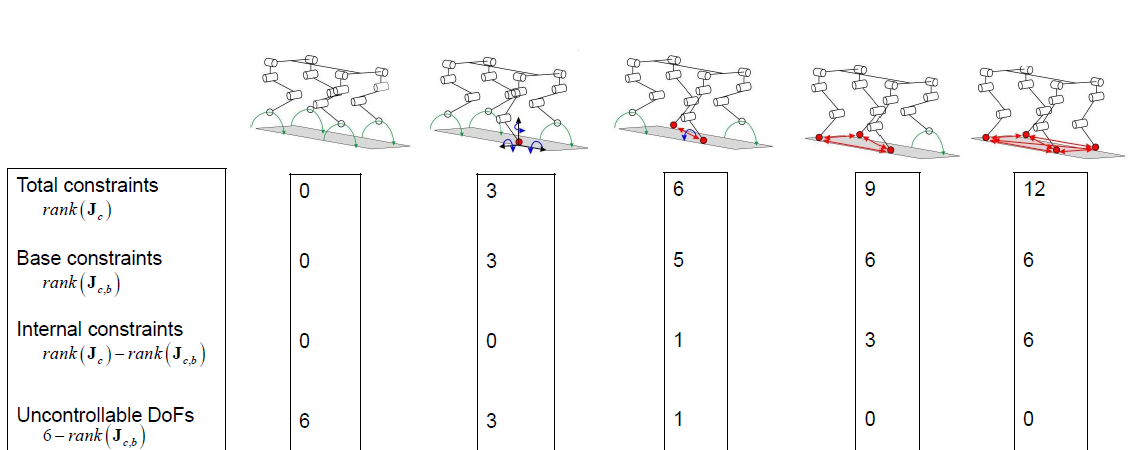
\includegraphics[width=1.05\linewidth]{images/Contraints_Quad.PNG}



\subsection{Support-consistent dynamics}
If we use {\bf soft contacts} to model the contact, we simply introduce an external force acting on the robot:
$${\bf F}_c = k_p({\bf r}_c - {\bf r}_{c0}) + k_d\dot{\bf r}_c$$
However such problems are hard to accurately solve numerically (slow system dynamics, fast contact dynamics). 

Instead it works better to use {\bf hard contacts}. We impose the kinematic constraint $\mvec{I}{J}{C_i}\dot{\bf u} + \mdvec{I}{J}{C_i}{\bf u} = \bm 0$ from above and calculate the resulting force and null-space matrix:
\begin{align*}
{\bf F}_c = ({\bf J}_c{\bf M}^{-1}{\bf J}_c^T)^{-1} ({\bf J}_c{\bf M}^{-1} ({\bf S}^T {\bf \tau - b - g}) + \dot{\bf J}_c{\bf u})\\
{\bf N}_c = \mathbb{I} - {\bf M}^{-1}{\bf J}_c^T({\bf J}_c{\bf M}^{-1}{\bf J}_c^T)^{-1}{\bf J}_c \\
\Rightarrow \boxed{   
{\bf N}_c^T({\bf M}\dot{\bf u} + {\bf b + g}) = {\bf N}^T_c {\bf S}^T {\bm \tau}, \quad {\bf J}_c{\bf N}_c = {\bf 0}  }
\end{align*}

By defining the \emph{end-effector inertia} $\bm\Lambda_c = ({\bf J}_c{\bf M}_c^{-1}{\bf J}_c^T)^{-1}$ we can write the kinetic energy loss on impact:
\begin{align*}
{\bf u}^+ &= {\bf N}_c{\bf u}^-\\
E_{loss} &= \Delta E_{kin} = - \frac 12 \Delta{\bf u}^T{\bf M}\Delta{\bf u} = - \frac 12 \dot{\bf r}^{-T}{\bf M}\dot{\bf r}^{-}
\end{align*}


\section{Dynamic control}

\subsection{Joint-space Dynamic Control}
$$\boxed{\mathbf{ M(q)\ddot{q} + b(q,\dot q) + g(q)} = 
\bm\tau}$$

Torque as a function of position and velocity error:
$${\bm \tau}^* = k_p({\bf q}^* - {\bf q}) + k_d(\dot{\bf q}^* - \dot{\bf q})$$

\textbf{Compensate for gravity} by adding an estimated gravity term:
$${\bm \tau}^* = k_p({\bf q}^* - {\bf q}) + k_d(\dot{\bf q}^* - \dot{\bf q}) + \hat{\bf g}({\bf q})$$

Compensate for \textbf{system dynamics}:
$$\bm\tau = \hat{\bf M}({\bf q})\ddot{\bf q}^* + \hat{\bf b}({\bf q}, \dot{\bf q}) + \hat{\bf g}({\bf q})$$

If the model is exact, we have $\mathbb{I}\ddot{\bf q} = \ddot{\bf q}^*$ (decoupled control), meaning we can perfectly control system dynamics. We could apply a PD-control law, making each joint behave like a mass-spring-damper with unitary mass:
$$\ddot{\bf q}^* = k_p({\bf q}^* - {\bf q}) + k_d(\dot{\bf q}^* - \dot{\bf q})$$
$$\omega = \sqrt{k_p}, \quad D = \frac{k_d}{2\sqrt{k_p}}$$

\newpage
\subsection{Task-space Dynamic Control}
$$\boxed{\dot{\bf w_{e}}
 =J_{e} \ddot{q} + \dot{J_{e}} \dot{q}=J_{e}M^{-1}(\tau - b -g)+\dot{J_{e}} \dot{q}}$$
 $$ \tau = J_{e}^{T}F_{e} \quad \textrm{,} \quad \ddot{q^*} = J_{e}^+ (\dot{\bf w_{e}}^* - \dot{J_{e}} \dot{{q}})$$ 
\subsection*{End-Effector Motion Control}
Generalized framework to control motion and force. \textbf{End-effector dynamics}:
\begin{align*}
\bm\Lambda \dot{\bf w}_e + \bm\mu + {\bf p} &= {\bf F}_e  \\
\bm\Lambda &= ({\bf J}_e{\bf M}^{-1}{\bf J}_e^T)^{-1} \\
\bm\mu     &= {\bm\Lambda}{\bf J}_e{\bf M}^{-1}{\bf b} - {\bm\Lambda}\dot{\bf J}_e\dot{\bm q} \\
{\bf p}    &= {\bm\Lambda}{\bf J}_e{\bf M}^{-1}{\bf g} \\
\end{align*}
represent the end-effector inertia, centrifugal/coriolis and gravitational terms in task space.\\
Following from the dynamics the \textbf{end-effector control} can be found:
$$\bm\tau^* = \hat{\bf J}^T(\hat{\bm\Lambda} \dot{\bf w}_e^* + \hat{\bm\mu} + \hat{\bf p})$$
$$\bf \dot{w}_{e}^* =k_{p}\begin{pmatrix} r_{e}^* -r_{e}\\ \Delta \phi_{e}\end{pmatrix}+k_{d}(w_{e}^* - w_{e})$$
$$ \Rightarrow \begin{pmatrix} r_{e}^* -r_{e}\\ \Delta \phi_{e}\end{pmatrix} =\begin{bmatrix}
\mathbb{1} & 0 \\ 0 & E_{R} \end{bmatrix}$$
$$\dot{\bf w}_e^* = k_p{\bf E}(\bm\chi^*_e \boxminus \bm\chi_e) + k_d({\bf w}_e^* - {\bf w}_e) \underbrace{+ \dot{\bf w}_e^*(t)}_\text{trajectory control} $$

\subsection*{Operational Space Control}
$$
\underline{{\bf F}_c} + \bm\Lambda \underline{\dot{\bf w}_e} + \bm\mu + {\bf p} = {\bf F}_e $$
$$
\bm\tau^* = \hat{\bf J}^T(\hat{\bm\Lambda} \underline{{\bf S}_M} \dot{\bf w}_e^* + \underline{{\bf S}_F{\bf F}_c} + \hat{\bm\mu} + \hat{\bf p})
$$\newline
with $S_{M}$ and $S_{F}$ being the selection matrices for Motion and Force. Let {\bf C} represent the rotation from the inertial frame to the contact force frame. The selection matrices can be calculated as (with $\sigma_{i} \in \{0,1\}$) :
\begin{align*}
\bm\Sigma_p &= \left[\begin{smallmatrix}
\sigma_{px} & 0 & 0 \\
0 & \sigma_{py} & 0 \\
0 & 0 & \sigma_{pz} \end{smallmatrix}\right], \;
\bm\Sigma_r = \left[\begin{smallmatrix}
\sigma_{rx} & 0 & 0 \\
0 & \sigma_{ry} & 0 \\
0 & 0 & \sigma_{rz} \end{smallmatrix}\right] \\
{\bf S}_M &= \left[\begin{smallmatrix}
{\bf C}^T\bm\Sigma_p{\bf C} & {\bf 0} \\
{\bf 0}  &  {\bf C}^T\bm\Sigma_r{\bf C}
\end{smallmatrix}\right]\\
{\bf S}_F &= \left[\begin{smallmatrix}
{\bf C}^T(\mathbb I - \bm\Sigma_p) {\bf C} & {\bf 0} \\
{\bf 0}  &  {\bf C}^T(\mathbb I - \bm\Sigma_r) {\bf C}
\end{smallmatrix}\right]
\end{align*}

\subsection*{OSC with multiple objectives}
Example: quadruped with three stationary legs and one in swing.
\begin{itemize}
\item Leg swing: $\ddot{\bf r}_{OF} = {\bf J}_F\ddot{\bf q}_F + \dot{\bf J}_F\dot{\bf q}_F = \ddot{\bf r}_{OF,des}(t) = k_p({\bf q
r}^* - {\bf r}) + k_d(\dot{\bf r}^* - \dot{\bf r}) + \ddot{\bf r}^*$
\item Body movement (translation and orientation): $\dot{\bf w}_B = {\bf J}_B\ddot{\bf q}_B + \dot{\bf J}_B\dot{\bf q}_B = \dot{\bf w}_{OB,des}(t) = k_p\begin{pmatrix}{\bf r}^* - {\bf r}\\ 
\bm \varphi^* \boxminus \bm \varphi
\end{pmatrix} + k_d({\bf w}^* - {\bf w}) + \dot{\bf w}^*$
\item Enforce contact constraints: $\ddot{\bf r}_c = {\bf J}_c\ddot{\bf q}_c + \dot{\bf J}_c\dot{\bf q}_c = {\bf 0}$
\end{itemize}
Solve for generalized acceleration and torque giving each task \textbf{equal priority}:
\begin{align*}
\ddot{\bf q}^* = \begin{bmatrix}
{\bf J}_F \\
{\bf J}_B \\
{\bf J}_c
\end{bmatrix}^+\left(
\begin{pmatrix}
\ddot{\bf r}_{OF,des}(t) \\
\dot{\bf w}_{B,des}(t)   \\
{\bf 0}
\end{pmatrix} - \begin{bmatrix}
\dot{\bf J}_F \\
\dot{\bf J}_B \\
\dot{\bf J}_c
\end{bmatrix} \dot{\bf q}
\right)
\end{align*}

Solve \textbf{with prioritization}:
\begin{align*}
\ddot{\bf q}^* =& \sum_{i=1}^{n_t}{\bf N}_i\ddot{\bf q}_i, \\
\ddot{\bf q}_i  \coloneqq&  ({\bf J}_j{\bf N}_i)^+ \left( {\bf w}_i^* - \dot{\bf J}_i\dot{\bf q} - {\bf J}\sum_{k = 1}^{i-1}{\bf N}_k\dot{\bf q}_k \right)
\end{align*}

Where ${\bf N}_i$ is the nullspace projection of ${\bf J}_i \coloneqq [{\bf J}_1^T \, ... \, {\bf J}_i^T]^T$.


\subsection{Inv. Dynamics Floating-Base}
Given a desired acceleration $\dot{\bf u^*}$ from the support-consistent dynamics follows:
%{\bm \tau}^* &= ({\bf N}^T_c {\bf S}^T )^+{\bf N}_c^T({\bf M}\dot{\bf u} + {\bf b + g}) \\
\begin{align*}
{\bm \tau}^* &= ({\bf N}^T_c {\bf S}^T )^+{\bf N}_c^T({\bf M}\dot{\bf u^*} + {\bf b + g}) \underbrace{+  \mathcal{N}({\bf N}^T_c {\bf S}^T)\bm\tau^*_0}_\text{multiple solutions}
\end{align*}

% --------------------- Commented out -----------------------
\begin{comment}
\subsection*{Quadratic minimization}
Least squares problems can be expressed in form of quadratic minimization problems. We can also perform multiple tasks with or without prioritization:
\begin{align*}
& \rightarrow \mathbf{Ax - b = 0} \Rightarrow \mathbf{x = A^+b} \\
&\Leftrightarrow \min_{\bf x}||\mathbf{Ax - b}||_2; \; \min_{\bf x}||{\bf x}||_2 \\
& \rightarrow \mathbf{A_1x_2 - b = A_2x_2} \Rightarrow \mathbf{\begin{pmatrix}
\bf x_1\\ \bf x_2
\end{pmatrix} = \begin{bmatrix}
\bf A_1 & \bf A_2
\end{bmatrix}^+b} \\
&\Leftrightarrow \min_{\bf x_1,x_2}\left\lVert\begin{bmatrix}
\bf A_1 & \bf A_2
\end{bmatrix}\begin{pmatrix}
\bf x_1\\ \bf x_2
\end{pmatrix} - b\right\rVert_2; \; \min_{\bf x_1,x_2}\left\lVert\begin{pmatrix}
\bf x_1\\ \bf x_2
\end{pmatrix}\right\rVert_2 \\
& \rightarrow \left\{ \begin{matrix}
\mathbf{A_1x = b_1}\\
\mathbf{A_2x = b_2}
\end{matrix}\right. \text{Equal priority} \Rightarrow {\bf x} = \begin{bmatrix}
{\bf A}_1 \\ {\bf A}_2
\end{bmatrix}\begin{pmatrix}
{\bf b}_1\\ {\bf b}_2
\end{pmatrix} \\
& \Leftrightarrow \min_{\bf x}\left\lVert\begin{bmatrix}
\bf A_1 \\ \bf A_2
\end{bmatrix}{\bf x} - \begin{pmatrix}
\bf b_1\\ \bf b_2
\end{pmatrix}\right\rVert_2; \; \min_{\bf x}||{\bf x}||_2 \\
& \rightarrow \left\{ \begin{matrix}
\mathbf{A_1x = b_1}\\
\mathbf{A_2x = b_2}
\end{matrix}\right. \text{Hierarchy} \Rightarrow \text{(nullspace projections)} \\
& \Leftrightarrow \min_{\bf x}\left\lVert 
{\bf A}_1{\bf x} - {\bf b}_1 \right\rVert_2; \; \left\{ \begin{matrix}
\min_{\bf x}\left\lVert {\bf A}_2{\bf x} - {\bf b}_2 \right\rVert_2 \\
\text{s.t. } \left\lVert {\bf A}_1{\bf x} - {\bf b}_1 \right\rVert_2 = c_1
\end{matrix}\right.
\end{align*}


\subsection*{OSC as quadratic program}
Rewrite the equations of motion and subsequent tasks as a prioritized sequence of quadratic minimization problems:
$$\min_{\bf x} ||{\bf A}_i{\bf x - b}_i||_2 \quad {\bf x} = \begin{pmatrix}
\dot{\bf u} \\ {\bf F}_c \\ {\bm \tau}
\end{pmatrix}$$
\end{comment}
% --------------------- Commented out -----------------------

\subsection*{Task-Space Control as QP}

The behaviour of a robotic system can be described as multi-task control problem with the optimization variable $x$ as follows:
$$ x_{fixed B}=\begin{pmatrix} \ddot{q} \\ F_{c} \\ \tau \end{pmatrix} \quad \textrm{or} \quad x_{floating B}=\begin{pmatrix} \dot{u} \\ F_{c} \\ \tau \end{pmatrix}$$\\
Using the optimization variable $x$ the EoM \newline $M\ddot{q}+b+g+J_{c}^{T}F_{c}=S^{T}\tau$ can be formulated as least square problem $Ax-b=0$:
$$A=\begin{bmatrix} \hat{M} & \hat{J_{c}^{T}} & -S^{T} \end{bmatrix} \quad \quad b=-\hat{b}-\hat{g}$$
To achieve a desired acceleration in the \textbf{joint space $\ddot{q}$} or at a point of interest in the \textbf{task space $J\ddot{q}+\dot{J}\dot{q}=\dot{\bf w_{e}}$}:
$$ A=\begin{bmatrix} \mathbb{I} \: \textrm{or} \: \hat{J_{i}} & 0 & 0 \end{bmatrix} \quad \quad b=\ddot{q} \: \textrm{or} \: \dot{\bf w_{e}^*}-\hat{J_{i}\dot{q}}$$\\
Pushing with a certain force $F_{i}=F_{i}^*$:
$$A=\begin{bmatrix} 0 & \mathbb{I} & 0 \end{bmatrix} \quad \quad b=F_{i}^*$$

\section{Legged Robots}
\subsection{Hierarchical Optimization}
Formulating a Hierarchical Optimization (HO) problem as a QP:
$$ \textrm{min}||A_{i}x-b_{i}||\quad \textrm{,} \quad C_{i}x\leq d_{i}$$\\
Achieved by following control scheme for robots:
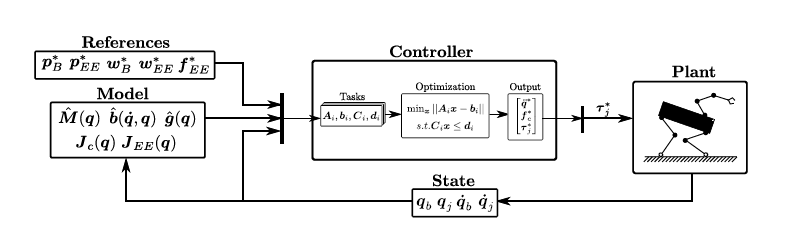
\includegraphics[width=1.05\linewidth]{images/Control_Legged.PNG}\\
The HO variable $x$ and EoM are defined as:
$$ M(q)\ddot{q}+b(q,\dot{q})+g(q)=S^{T}\tau_{j}+J_{c}^T(q)f_{c}$$
$$x= [\ddot{q}^T \quad f_{c}^T \quad \tau_{j}^T ]^T$$
Task 1: Fulfill equation of Motion:
$$ A_{1}=[M(q) -J_{c}^T -S^T] \quad \textrm{,} \quad b_{1}=-b-g$$
Task 2: Ensure feet stationary on ground:
$$ A_{2}=[J_{c,lin} \quad 0 \quad 0] \quad \textrm{,} \quad b_{2}=\dot{\bf w_{c}^*}-\dot{J_{c,lin}}\dot{q}$$
Task 3: Move body accord ref. trajectory:
$$ \dot{ w_{B}^*}=k_{p}(p_{B}^*-p_{B})+k_{d}(w_{B}^*-w_{B} $$
$$ A_{3}=[J_{B} \quad 0 \quad 0] \quad \textrm{,} \quad b_{3}=\dot{w_{B}^*}-\dot{J_{B}}\dot{q} $$
\textbf{...To be continued...}
\section{Rotorcraft}

Propeller thrust and drag proportional to squared rotational speed ($b$: thrust constant; $d$: drag constant):
$$T_i = b\omega_{p,i}^2, \quad Q_i = d\omega_{p,i}^2$$


\subsection{Kinematics}

Use Tait-Bryan angles, consisting of yaw $\psi$ (Z-axis), pitch $\theta$ (Y-axis) and roll $\phi$ (X-axis). 
$${\bf C}_{EB} = {\bf C}_{E1}({\bf z}, \psi) \cdot {\bf C}_{12}({\bf y}, \theta) \cdot {\bf C}_{2B}({\bf x}, \phi)$$
Angular velocity:
\begin{align*}
\mvec{B}{\omega}{} &= \mvec{B}{\omega}{\text{roll}} + \mvec{B}{\omega}{\text{pitch}} + \mvec{B}{\omega}{\text{yaw}}\\
\mvec{B}{\omega}{\text{roll}} &= (\dot\psi, 0, 0)^T\\
\mvec{B}{\omega}{\text{pitch}} &= {\bf C}_{2B}^T(0,\dot\theta, 0)^T\\
\mvec{B}{\omega}{\text{yaw}} &= [{\bf C}_{12}\cdot {\bf C}_{2E}]^T (0, 0, \dot\phi)^T \\
\mvec{B}{\omega}{} &= J_r\dot{\bm \chi}_r = J_r \begin{pmatrix}
\dot\phi\\
\dot\theta\\
\dot\psi
\end{pmatrix} \\
J_r &= \begin{bmatrix}
1 & 0 & -\sin\theta \\
0 & \cos\phi  &  \sin\phi\cos\theta \\
0 & -\sin\phi  &  \cos\phi\cos\theta
\end{bmatrix}\overset{\theta=\phi=0}{=}\mathbb{I}_{3x3}
\end{align*} \newline

NB: singularity for $\theta = \pm \ang{90}$ (Gimbal lock).


\subsection{Dynamics}
$$\boxed{ M(\varphi)\ddot{\varphi}+b(\dot{\varphi},\varphi)+g(\varphi)+J_{ext}^T F_{ext}=S^T\tau_{act}}$$
Change of momentum and spin in the body frame (${\bf M} = $ total moment/torque):
$$\begin{bmatrix}
m\mathbb{I} & 0\\
0 & {\bf I}
\end{bmatrix}\begin{bmatrix}
\mdvec{B}{v}{} \\
\mdvec{B}{\omega}{}
\end{bmatrix} + \begin{bmatrix}
\mvec{B}{\omega}{} \times m \mvec{B}{v}{} \\
\mvec{B}{\omega}{} \times {\bf I}\mvec{B}{\omega}{}
\end{bmatrix} = \begin{bmatrix}
\mvec{B}{F}{}\\ \mvec{B}{M}{}
\end{bmatrix}
$$
$$ \begin{bmatrix} \dot{x} \\ \dot{y}\\ \dot{z} \end{bmatrix}=C_{EB}v=C_{EB}\begin{bmatrix} u\\ v\\ w\end{bmatrix} $$
%$$ E_{R}\begin{bmatrix} \dot{\phi}\\ \dot{\theta} \\ \dot{\psi} \end{bmatrix}=\omega=\begin{bmatrix} p \\ q \\ r\end{bmatrix}$$
Forces and moments come from gravity and aerodynamics:
\begin{align*}
\mvec{B}{F}{} &= \mvec{B}{F}{G} + \mvec{B}{F}{Aero} \\
\mvec{B}{M}{} &= \mvec{B}{M}{Aero} \\
\mvec{B}{F}{G} &= \mathbf{C}_{EB}^T \begin{bmatrix}
0 \\ 0 \\ mg
\end{bmatrix} \\
\mvec{B}{F}{Aero} &= \sum_{i=1}^4 \begin{bmatrix}
0 \\ 0 \\ -T_i = -b{\bf \omega}_{p,i}^2
\end{bmatrix}\\
\mvec{B}{M}{Aero} &= \mvec{B}{M}{T} + \mvec{B}{Q}{} =\\ \quad & \quad  \begin{bmatrix}
l(T_4 - T_2) \\
l(T_1 - T_3) \\
0
\end{bmatrix} + \begin{bmatrix}
0 \\ 0 \\ \sum_{i=1}^4 Q_i(-1)^{(i-1)}
\end{bmatrix}
\end{align*}\\

Full control over all rotational speeds, independently of the current position state. \textbf{Only directly control of vertical cartesian velocity - attitude control must be used for full position control.}

\subsection{Control}

\textbf{Movement directions with four propellers:}

\begin{center}
    
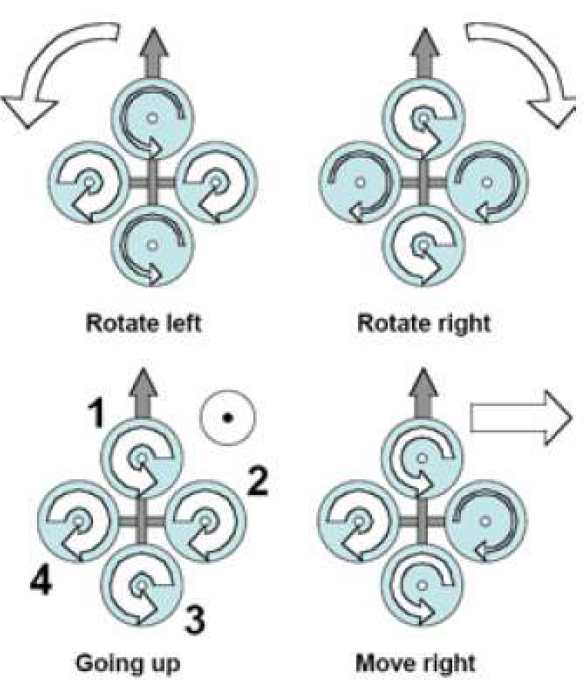
\includegraphics[width=0.7\linewidth]{images/RC_MovingDirections.PNG}\\
\end{center}
\textbf{Possible Control Structures:}
\begin{center}
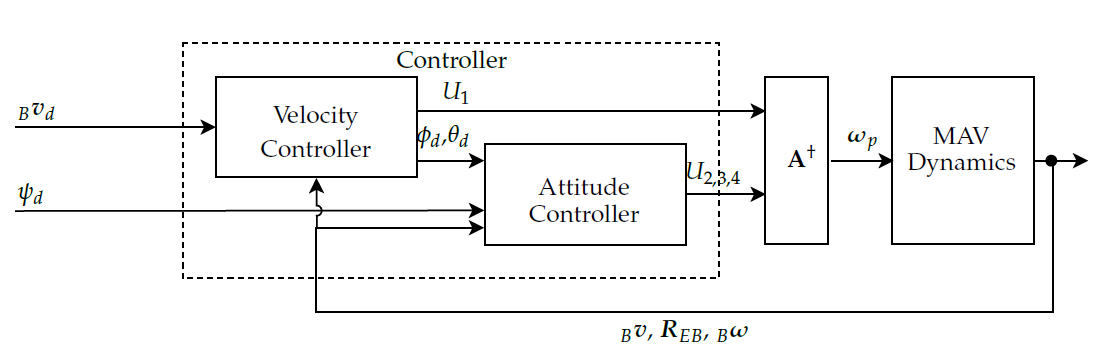
\includegraphics[width=1\linewidth]{images/RC_Control_Structure1.PNG}\\
    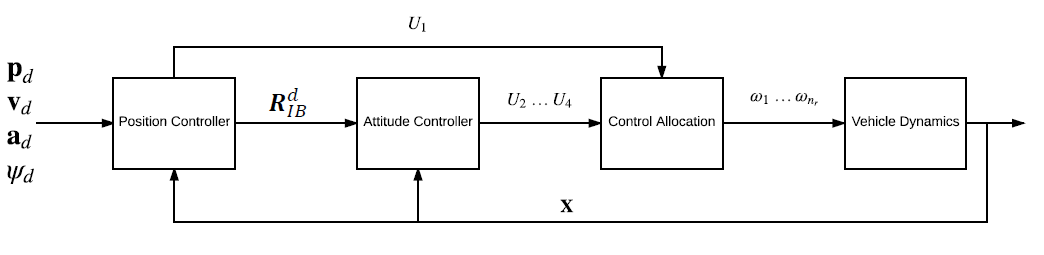
\includegraphics[width=1\linewidth]{images/RC_Control_Structure2.PNG}
\end{center}
To formulate the control architecture, a virtual control input $U$ is used:
$$ \begin{pmatrix}
U_1 \\U_2 \\U_3 \\U_4 
\end{pmatrix}=A\begin{pmatrix}
\omega_{1}^2 \\
\vdots \\
\omega_{i}^2
\end{pmatrix} \quad \textrm{,} \quad A^{\dagger}= A^T(AA^T)^{-1}
$$\\
Hence the translational and rotational dynamics are stated as follows:
\begin{align*}
\dot{p} &= R_{EB} \mvec{B}{v}{}\\
\mvec{B}{\dot{v}}{} &=-\omega \times \mdvec{B}{v}{}+\begin{pmatrix}
0 \\ 0 \\ \frac{U_{1}}{m}
\end{pmatrix}+R_{EB}^T g\\
\dot{R}_{EB} &= R_{EB} \omega\\
\dot{\omega} &= J^{-1}(-\omega \times J\omega+\begin{pmatrix}
U_2 \\ U_3 \\ U_4
\end{pmatrix}
)
\end{align*}
\textbf{Equilibrium Point:}\\
$$ \phi=\theta=p=q=r=0 \; \textrm{;} \; U_2=U_3=U_4=0$$

$$U_{1}=mg\\
sin(x) \approx x \; \textrm{,} \; cos(x) \approx 1$$\\
This results in following Control Inputs:
\begin{align*}
    U_1 &= T_{des}\\
    U_2 &= (\phi_{des}-\phi)k_{pRoll}-\dot{\phi}k_{dRoll}\\
    U_3 &= (\theta_{des}-\theta)k_{pPitch}-\dot{\theta}k_{dPitch}\\
    U_3 &= (\psi_{des}-\psi)k_{pYaw}-\dot{\psi}k_{dYaw}\\
\end{align*}

\textbf{...Velocity or Position Control...}


\subsection{Propeller aerodynamics}
Propeller in hover:
\begin{itemize}
\item Thrust force $T$ normal to prop. plane, $|T| = \frac{\rho}{2} A_P C_T(\omega_p R_p)^2$
\item Drag torque $Q$, around rotor plane $|Q| = \frac{\rho}{2} A_P C_Q(\omega_p R_p)^2R_p$
\item $C_T$ and $C_Q$ depend on blade pitch angle (prop geometry), Reynolds number (prop speed, velocity, rotational speed).
\end{itemize}

Propeller in forward flight: additional forces due to force unbalance between forward- and backward-moving props.
\begin{itemize}
\item Hub force $H$ (orthogonal to $T$, opposite to horizontal flight direction $V_H$), $|H| = \frac{\rho}{2} A_P C_H(\omega_p R_p)^2R_p$
\item Rolling torque $R$ around flight direction $|R| = \frac{\rho}{2} A_P C_R(\omega_p R_p)^2R_p$
\item $C_R$ and $C_H$ depend on advance ratio $\mu = \frac{V}{\omega_P R_P}$
\end{itemize}

Ideal power consumption at hover: $P = \frac{F_{Thrust}^{3/2}}{\sqrt{2\rho A_R}} = \frac{(mg)^{3/2}}{\sqrt{2\rho A_R}}$. The prop efficiency is measured with the Figure of Merit FM:
$$FM = \frac{\text{Ideal power to hover}}{\text{Actual power to hover}} < 1$$

Blade Elemental and Momentum Theory (BEMT): blade shape determines drag and lift coefficients $c_D$, $c_L$.




\section{Fixed-Wing}
\subsection{Aerodynamic Basics}
\begin{center}
    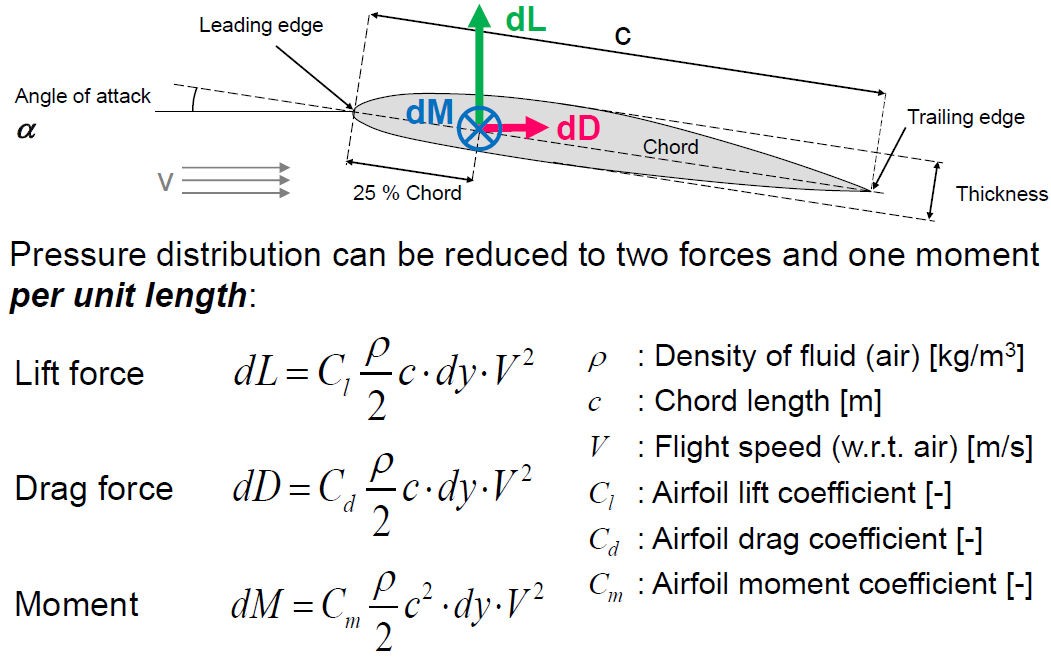
\includegraphics[width=1\linewidth, frame]{images/UAV_Airfoil.PNG}
\end{center}
Stall does highly depend on fluid, foil and Reynolds number:
\begin{center}
    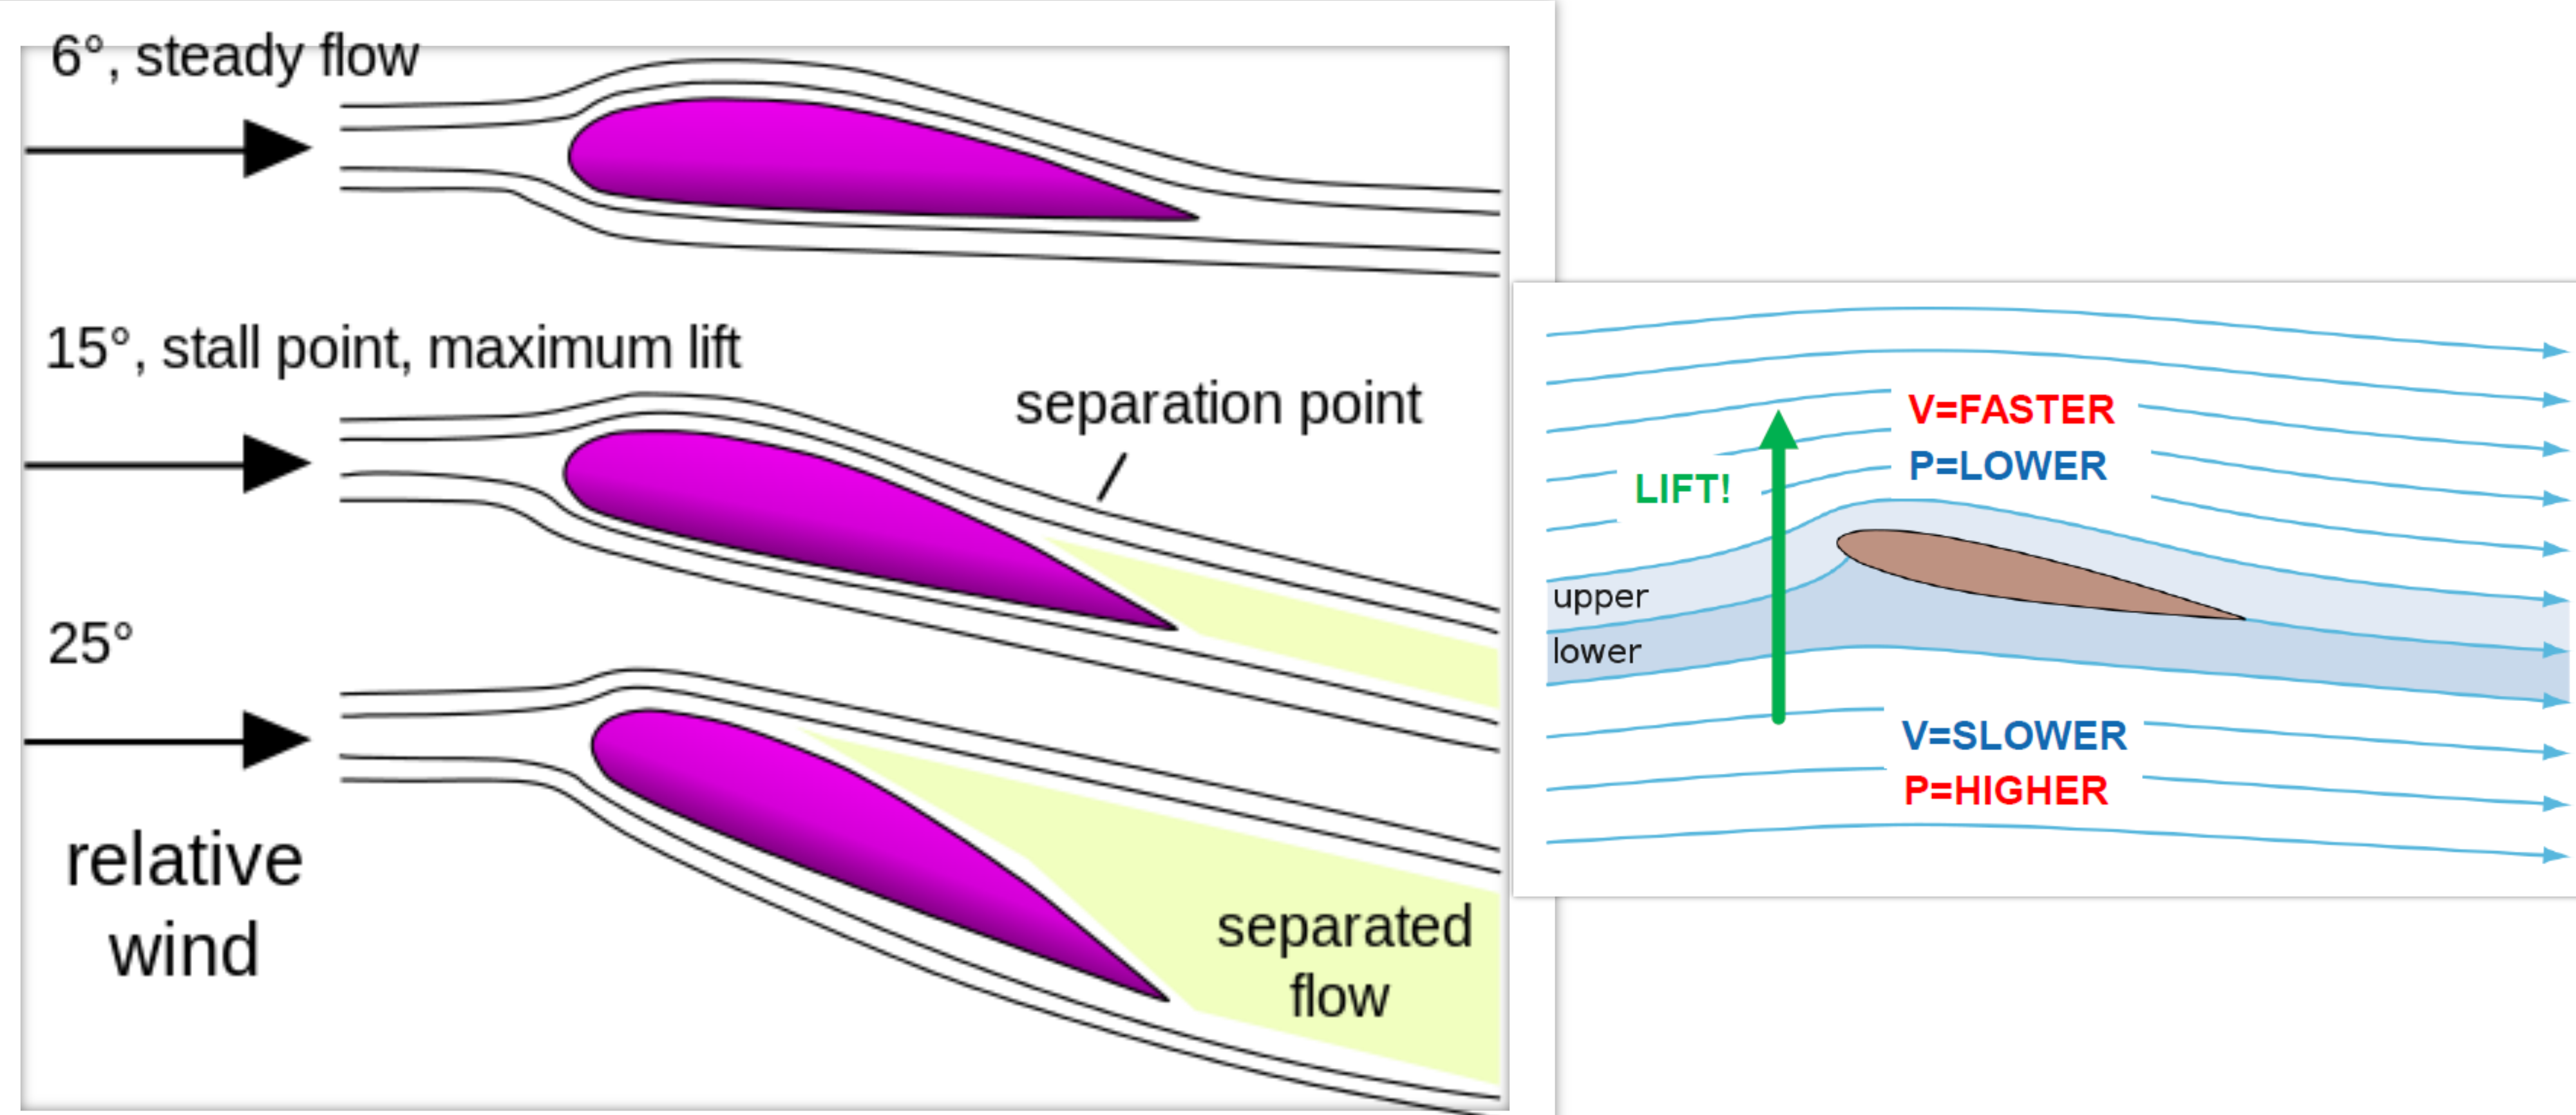
\includegraphics[width=1\linewidth]{images/FW_Stall.png}
\end{center}
Small FW provide following control surfaces:
\begin{center}
    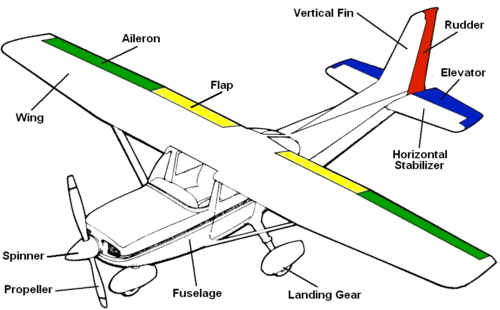
\includegraphics[width=0.7\linewidth]{images/FW_Control.png}
\end{center}




\subsection{Kinematics}
\textbf{Body-axis $\mathcal{B}$}\\
Body velocity: $\mvec{\mathcal{B}}{v}{a}=(u,v,\omega)^T$\\
Body rates: $\mvec{\mathcal{B}}{\omega}{}=(p,q,r)^T$\\
Air-mass relative speed (airspeed): $V=\sqrt{u^2+v^2+\omega^2}$\\
\textbf{Wind-axis $\mathcal{W}$}\\
Angle of attack: $\alpha=tan^-1(\omega/u)$\\
Sideslip angle: $\beta=sin^-1(v/V)$\\
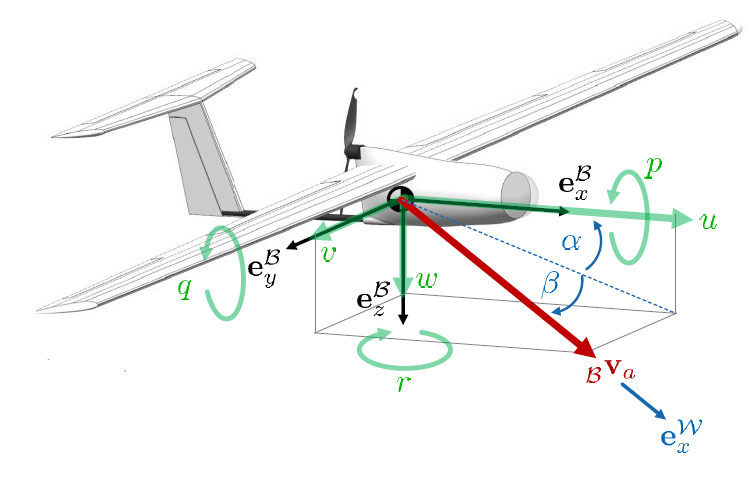
\includegraphics[width=1\linewidth]{images/FW_KinematicOverview.PNG}
\textrm{Polar Coordinates}\\

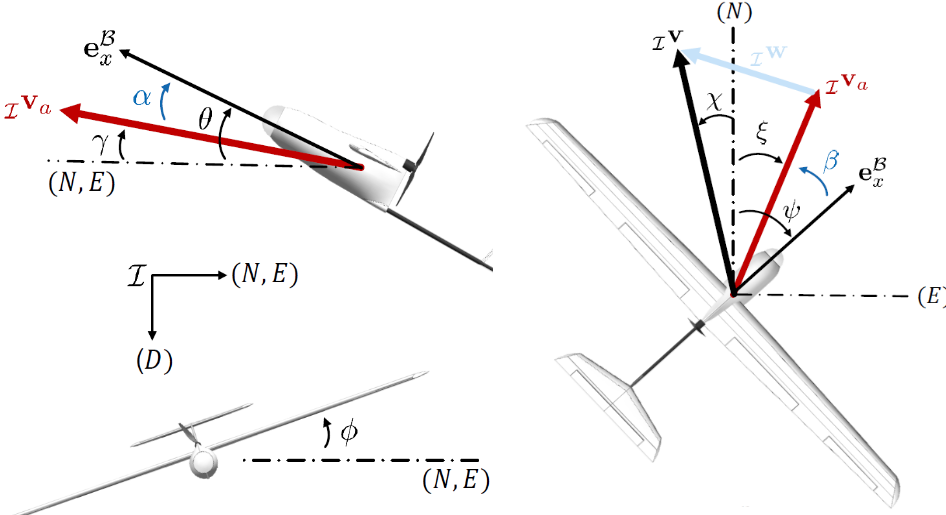
\includegraphics[width=1\linewidth]{images/FW_Angles.png}
$\gamma$: Flight path angle from horizon\\
$\theta$: Pitch anlge from horixon to $x$\\
$\phi$: Roll angle, rotation about $x$\\
$\xi$: Heading angle, from North\\
$\psi$: Yaw angle, from North\\
$\chi$: Course angle from North\\
$\mvec{\mathcal{I}}{v}{}$: Ground based internal velocity / ground speed)\\

$\mvec{\mathcal{I}}{v}{a}=C_{\mathcal{IB}}\mvec{\mathcal{B}}{v}{a}$
$\mvec{\mathcal{I}}{v}{}=\mvec{\mathcal{I}}{v}{a}+\mvec{\mathcal{I}}{w}{}=\mvec{\mathcal{I}}{\dot{r}}{}=\begin{bmatrix}
V\cos{\gamma}\cos{\xi}+\omega_{N}\\
V\cos{\gamma}\sin{\xi}+\omega_{E}\\
-V\sin{\gamma}+\omega_{D}
\end{bmatrix}$


\subsection{Dynamics}
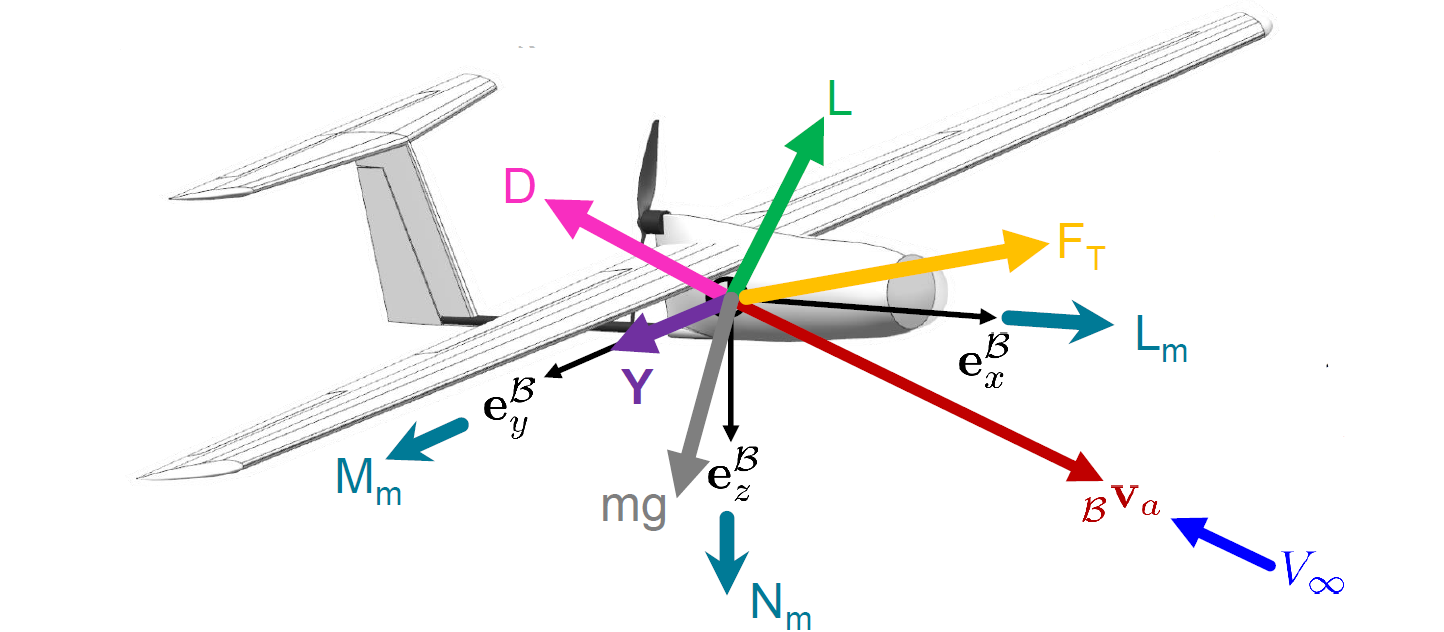
\includegraphics[width=1\linewidth]{images/FW_Dynamics.PNG}
Lift $L=\frac{1}{2}\rho V^2Sc_{L}$\\
Drag $D=\frac{1}{2}\rho V^2 S c_{D}$\\
Rolling Moment $L_{m}=\frac{1}{2}\rho V^2 S b c_{l}$\\
Pitching Moment $M_{m}=\frac{1}{2}\rho V^2 S \overline{\rm c} c_{m}$\\
Yawing Moment $N_{m}=\frac{1}{2}\rho V^2 S b c_{n}$\\
\newline

\textbf{EoM Translation}
\begin{align*}
    \dot{u} &= rv-qw+\frac{1}{2}(F_{T}\cos{\epsilon}-D\cos{\alpha}+L\sin{\alpha})-g\sin{\theta}\\
    \dot{v} &=pw-ru+\frac{1}{m}Y+g\sin{\phi}\cos{\theta}\\
    \dot{w} &=qu-pv+\frac{1}{m}(F_{T}\sin{\epsilon}-D\sin{\alpha}-L\cos{\alpha})+g\cos{\phi}\cos{\theta}\\
    \begin{bmatrix} \dot{x} \\ \dot{y} \\ \dot{z} \end{bmatrix} &= C_{IB}\begin{bmatrix}
    u\\v\\w \end{bmatrix}+\mvec{\mathcal{I}}{w}{}
\end{align*}

\textbf{EoM Rotation (Assumed $I_{xz} \approx 0$ }
\begin{align*}
    \dot{p} &= \frac{1}{I_{xx}}(L_{m}+L_{m_{T}}-qr(I_{zz}-I_{yy}))\\
    \dot{q} &= \frac{1}{I_{yy}}(M_{n}+M_{m_{T}}-pr(I_{xx}-I_{zz}))\\
    \dot{r} &= \frac{1}{I_{zz}}(N_{m}+N_{m_{T}}-pq(I_{yy}-I_{xx}))\\
    \begin{bmatrix} \dot{\phi} \\ \dot{\theta} \\ \dot{\psi}
    \end{bmatrix} &= J_{r}^{-1}\begin{bmatrix}
    p \\ q \\ r
    \end{bmatrix} = \begin{bmatrix}
    p+q\tanh{\theta}\sin{\phi}+r\tan{\theta}\cos{\phi}\\
    q\cos{\phi}-r\sin{\phi}\\
    q\frac{\sin{\phi}}{\cos{\theta}}+r\frac{\cos{\phi}}{\cos{\theta}}
    \end{bmatrix}
\end{align*}

\subsection{Control}
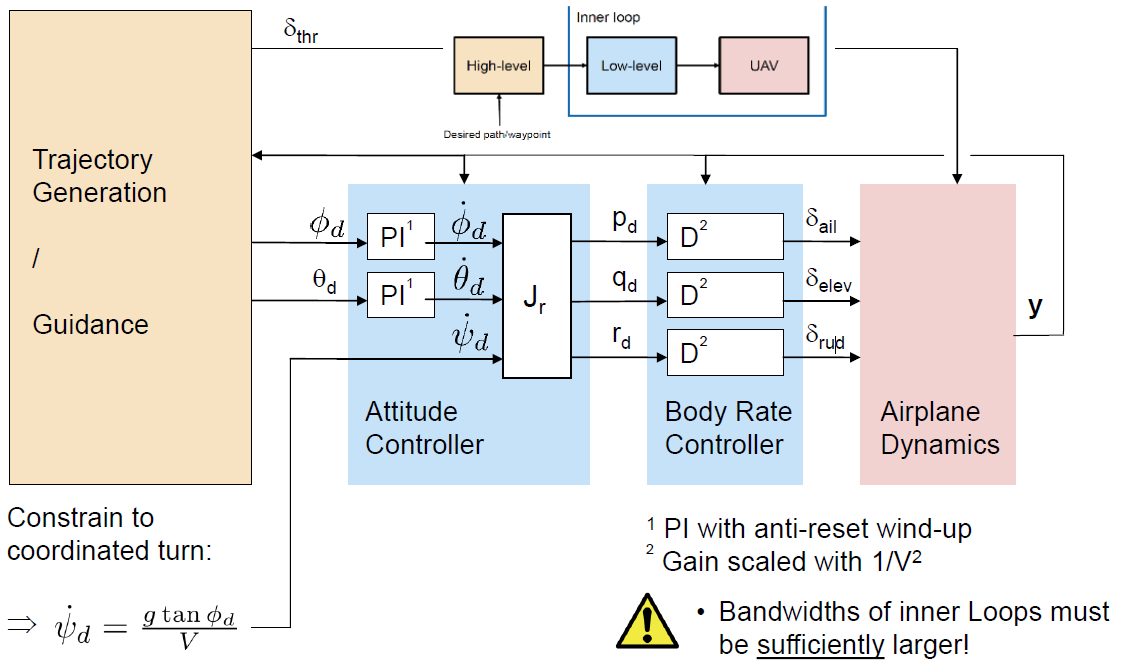
\includegraphics[width=1\linewidth]{images/FW_ControlLoop.png}\\
\textbf{Steady level turning flight}
$\mvec{\mathcal{B}}{\dot{v}}{a}=\mvec{\mathcal{B}}{\dot{\omega}}{}=0$ Steady (unaccelerated)\\
$\theta=\alpha \rightarrow \gamma =0 \textrm{Level}$\\
$\phi=\textrm{const.}\neq 0 \textrm{Turning}$\\
$\xi=\psi \textrm{No Sideslip}$\\
$Y=0$ Coordinated turn\\
$L$ increases with $\frac{1}{\cos{\phi}}$\\
$V_{min}$ increases with $\sqrt{\frac{1}{\cos{\phi}}}$\\
From Force balance and assumption $\dot{\psi} \approx \dot{\xi}$






%\subsection*{Support-consistent dynamics}
%\begin{itemize}
%\item EoM cannot be used directly due to external contact forces
%\item Contact force: \\ ${\bf F}_c = ({\bf J}_c{\bf M}^{-1}{\bf J}_c^T)^{-1} ({\bf J}_c{\bf M}^{-1} ({\bf S}^T {\bf \tau - b - g}) + \dot{\bf J}_c{\bf u})$
%\item Null-space projection \\ ${\bf N}_c = \mathbb{I} - {\bf M}^{-1}{\bf J}_c^T({\bf J}_c{\bf M}^{-1}{\bf J}_c^T)^{-1}{\bf J}_c$
%\item Support-consistent dynamics ${\bf N}_c^T({\bf M}\dot{\bf u} + {\bf b + g}) = {\bf N}^T_c {\bf S}^T {\bm \tau}$
%\item Inverse dynamics (may have multiple solutions): \\
%$ {\bm \tau}^* = ({\bf N}^T_c {\bf S}^T)^+({\bf N}_c^T({\bf M}\dot{\bf u} + {\bf b + g})) + \mathcal{N}({\bf N}^T_c {\bf S}^T){\bm \tau}^*_0 $
%\end{itemize}





\end{multicols*}



\end{document}